% My Preamble
\documentclass[12pt, letterpaper]{article}
% unless you are not sure do not change this from default
\usepackage[utf8]{inputenc}

\title{My First LATEX Document}
% Thanks always comes under inside author to acknowledge others.
\author{Anubhav Kumar \thanks{Funded by me and IITR}}
% We can use the \today to always update the document with the latest date or can specify the date we want to be.
\date{\today}

% To include the images we have to use packages graphicx
\usepackage{graphicx}
% setting the images storage location
\graphicspath{ {images/} }

% For using math we need a powerful package which extends the functionality of the inbuilt math.
\usepackage{amsmath}

% Lets define the body of the Tex
\begin{document}
% \maketitle can also come in between the document as per requirements.
\maketitle

This is my first Latex document and its already late i have to complete ASAP.
The upper part above the begin block is called preamble.
\% before a line is used here as a comment.
My performance has not \textbf{very bad} this academic year this can \underline{negatively affect} my relationship with my guides so i have to start working on some \textbf{\emph{A.I} application} to get back the reputation \textit{otherwise you will \emph{lag} behind from others in terms of good connections.}
% emph can alson be used which will italized a word in noraml text and vice versa.

This is how i look in figure \ref{fig:my_label}, in page \pageref{fig:my_label}. 
% using the same label my_label to insure we are referring the right label while using in TEXT.
But now moving this to a figure environment which should be a standard practice and width should always be define in includegraphics as it will not go out of page.

\begin{figure}[h]
    \centering
    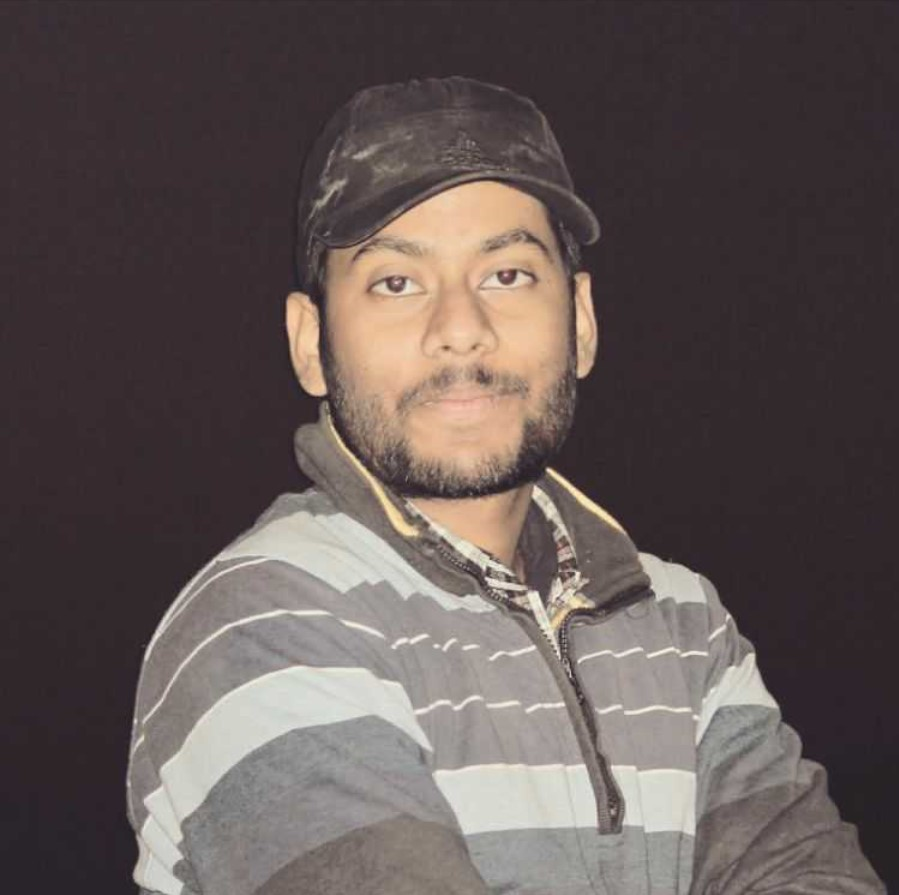
\includegraphics[width=0.5 \textwidth]{anubhav}
    \caption{This is me.}
    \label{fig:my_label}
\end{figure}

% Going for list which represent data in ordered fashion eg bullet.
\textbf{What is relationship conclusions in un-ordered list?}
\begin{itemize}
    \item This all will be printed in an un-ordered manner which will use \textbf{\emph{bullets}} and it will be printed without any numbers but text length can be as long as you want. 
    \item One long term relationship keeps your focus on your goals and gives meaning to one's life. It brings out best character from your mind and prepares you for other life's challenge.
    \item Many short encounters only consumes your energy and distract you from discovering yourself. So don't focus on these encounters but there is a silver lining as you should not put all your eggs in one basket so at least you should in a situation that you can adjust to different situations.
    \item And When you have your partner fully comfortable with you, you have the greatest support available to you not only in adverse situations when you are down but also when you are going through tough times.
\end{itemize}

% same syntax is used for ordered list but it in a different environment.
\textbf{What is the ordered list then?}
\begin{enumerate}
    \item This list uses the enumerate env against the itemize to form the ordered list with no which automatically increments.
    \item This list will be starting from 1 and will auto increment.
    \item Calling them list is somewhat relate able to a programming language.
\end{enumerate}

\textbf{Adding MATH to LATEX env.}
\begin{enumerate}

\item Math or equation can be written in two modes one is display mode where the equation is written in separate complete line where inline mode is used for writing math within the text.
\item My favourite equation in inline mode using \$..inline equation..\$ in $E=mc^2$ in which E is the energy desire, m is property of the tested object, and c is velocity or difficulty to catch it. So Einstein's equation hold true in many forms Below is this equation in display form.
\[E=mc^2\]
\item If the difficulty is min (\begin{math} c=1 \end{math}) then the energy only depends on the properties of tested subject. And hence the modified equation reduces to below display form.
% equation env is part of amsmath package
\begin{equation}
    E=m
\end{equation}
\item Using equation env from amsmath package is not only the best method but it automatically marks the equation no also.
\begin{equation}
    For-developed-mind: Desire = m*(difficulty)^2
\end{equation}
\item amsmath package also provides a lot of the other handy tools so it should be by default included into every document.
\item Subscripts can be written using underscore in any math env as \emph{$A_nubhav$} and super script can be written using \^ character \textbf{$A^nuvhab$} but here only the immediate following character is affected. This can be nested like

\[ T^{i_1 i_2 \dots i_p}_{j_1 j_2 \dots j_q} = T(x^{i_1},\dots,x^{i_p},e_{j_1},\dots,e_{j_q}) \]

\item We write integrals by \\int and like $\int$ and fractions using \\frac{a}{b} like $\frac{a}{b}$. Limits on the integral can be placed using the sub and super scripts.Below is an example of integral by part.

\[\int_0^1 \frac{dx}{e^x} = \frac{e-1}{e} \]

\item Lower case Greek letter starts with lowercase like omega $\omega$ while uppercase with Delta $\Delta$.

\item Trigonometric and mathematical operator are prefixed with backslash like \\sin alpha $\sin(\alpha)$ $\cos(\beta)$ and $\log(x)$

\item Double Backslash cause a line break in paragraph while other with backslash prints on screen observe above line for an example.

\end{enumerate}
Really the possibilities with math in LATEX functions are limitless and it is just the tip of the iceberg so more exploration can be done as there comes the requirements.

\textbf{\emph{This completes a basic overview of the LATEX in a different source we are going to learn about BASIC FORMATTING. } }
\end{document}